
\section{van Emde Boas trees}

We shall first introduce the so-called \textit{van Emde Boas}\index{van Emde Boas} trees which support dictionary\index{Dictionnary}-like operations in $O(\log \log N)$ worst-case time. But it requires that the elements are integers within the range $0$ to $N-1$, with no duplicates allowed. As it will introduce some confusions, we will redefine some notions:

\begin{itemize}
    \item We will denote the set of possibles integers as the universe $U$: $\left\{ 0, 1, ..., u - 1\right\}$.
    \item $u$ will be the universe size, and is often intented to be a power of two $2^{w}$ where $w$ is understood as the word size defined in word-RAM models.
\end{itemize}

This data structure behaves like a set but owns two main other operations: the predecessor ($\text{max}(\left\{e | e < x, e \in S\right\}$) and the successor; it can thus be used as a dictionary\index{Dictionnary} or a priority queue~\cite{van1976design}. But it consumes a lot of memory $O(u)$.

We will present it in a different fashion than the one used by van Emde Boas et al.~\cite{van1976design} but in the way that we can retrieve it by Cormen et al.~\cite{cormen2009introduction}.

\subsection{Direct mapping \& stratified tree}

With a really huge amount of memory, we could save all the elements of the set as a bit array where the $i$th position determines whether the $i$ element is set. This grants natural $O(1)$ for membership testing, insert and delete operations but finding the predecessor or successor could lead to $\Theta(u)$.

We can cut the space search for predecessor/successor by constructing a tree such that the node is marked as $1$ if none of its children is $0$ and $0$ otherwise (see Figure \ref{fig:vEB}). The membership is still in $O(1)$ but all the other operations became potentially $O(\log u)$. The idea consists to bound the height of the tree which will fix the amount of recursion and thus the complexity. van Emde Boas~\cite{van1977preserving} came up, in 1977, with the solution to decompose the problem in \textit{clusters} divided in $m$ \textit{galaxies} of size $k$. This cluster will be used to sum up the information of the whole subtree. One can remark that we can easily determine in which tree the element will go based on its index $\lfloor \frac{x}{k} \rfloor$.

Now, to achieve the $O(\log \log u)$, we need to cut recursively the space in cluster of $O(\sqrt{u})$. This leads to: $T(u) \leq T(\sqrt{u}) + O(1) \leadsto T(u) = O(\log \log u)$. Then, we will have to ensure that the algorithms do not need to perform two recursions, which would lead to $O(\log u)$ instead of $O(\log \log u)$, we must absolutely recurse on one and unique path in the tree. We will also remark that this structure has a lot of historical background~\cite{van2013thirty}.

\begin{figure}[!h]
   \caption{Stratified tree}
   \label{fig:vEB}
   \centering
   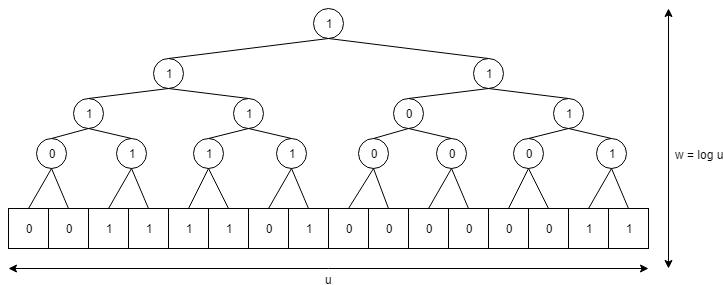
\includegraphics[width=0.9\textwidth]{stratified-tree.png}
\end{figure}

\subsubsection{van Emde Boas trees}

The van Emde Boas\index{van Emde Boas} trees is a data structure which can be seen as a tree with high degree and defined recursively. It is composed of two elements:
\begin{itemize}
    \item Clusters: Each cluster holds $\sqrt{u}$ subclusters and this recursively until it contains all the elements of the universe.
    \item Summary: Each cluster is summarized by one element which will help to guide the path to the predecessor or successor element. It is also recursively defined since the summary summarizes the information of its subtree.
\end{itemize}

The whole point is that we can access these helper structures in constant time due to the definition of our tree where the index of the cluster can be easily computed at each step. Hence, the cluster and its relative offset is defined as $(\frac{x}{\sqrt{u}}, x \text{ mod } \sqrt{u})$ which in the case of binary numbers leads to: $(\frac{x}{2^{\frac{w}{2}}}, x \text{ mod } 2^{\frac{w}{2}})$ which are roughly a shift and a mask operations.

\begin{figure}[!h]
   \caption{vEB idea}
   \label{vEB}
   \centering
   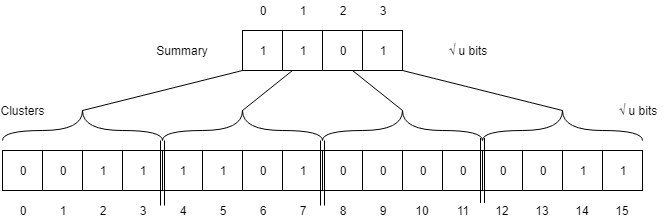
\includegraphics[width=0.9\textwidth]{vEB.png}
\end{figure}

K. Melhorn and S. Näher~\cite{mehlhorn1990bounded} proved that we can achieve $O(N)$ memory if we use hash tables\index{Hash table} which map prefix of the integers to ordered linked-list nodes while preserving complexity with high probability. An idea similar to Y-fast tries can also be applied for this purpose.

\subsection{X/Y-fast tries}

The problem with the \textit{van Emde Boas}\index{van Emde Boas} trees is that they consume a huge amount of memory. D. E. Willard~\cite{willard1983log}, in 1982, proposed two solutions to this problem based on the stratified tree idea. The first part of its answer is called the \textit{X-fast} trie, the idea is rather simple, only store the present elements, whose bit are set to one. We save the path to the node (with left as 0 and right as 1, for example) in a dynamic hash table, called level-search structure, and we associate it with the minimal/maximal value of the subtree. So instead of directly jumping to the subtree, we ensure the presence thanks to the hash table. This technique consumes $O(N \log u)$ memory to store each elements and their binary representation (note that we can spare some space since a common prefix/suffix is shared). Also, we may need to update a whole path, up to $O(\log u)$ values but we can achieve predecessor/succesor queries in $O(\log \log u)$ with high probability and search for one specific elements in $O(1)$. We can also maintain a linked list of the entire set of occupied leaves, this allows that given node x, we can find the successor and the predecessor in $O(1)$.

Second, we gain a lot of space, but we lose the $O(\log \log u)$ on insert and delete. Hopefully, the \textit{Y-fast} trie are there. They consist of two layers, the summit of the trie is made of a \textit{X-fast} trie such that it holds $\Theta(\frac{N}{\log u})$ elements and the leaves are other canonical binary seach trees of $O(\log u)$ elements where one representant is placed in the upper trie. This thus achieves the $O(N)$ in space and the operations are bound by $O(\log \log u)$ in the bottom trees since the update time is dominated by the leaf structures. Complexity is exchanged throughout the structure by amortizing it into the terminal elements.

Finally, let's conclude by saying that this data structure even though has nice properties, we may prefer to implement a \textit{X-fast} trie which are simpler to code and more efficient in practice. We need also to emphasize on the fact that the performances of this tree depends heavily on the hash table performances and the time to insert one element can thus vary by a huge factor. Notice that the complexity is not optimal, it is expected to be $O(\frac{\log \log u}{\log \log \log u})$ for $N^{O(1)}$ space~\cite{patracscu2007randomization}. Other data structures based on similar concepts have been developed to address the problem of the predecessor or the dynamic least common ancestor~\cite{bose2013fast,belazzougui2009monotone}. You may also be interested in the little brother of this data structure, defined in the $AC^{0}$ computation model (constant depth circuit which behaves as word-RAM like without multiplication), and called \textit{fusion tree}~\cite{fredman1990blasting}.